\documentclass[11pt,a4paper,ngerman]{report}
% sostituire con report/book per il formato elettronico

\usepackage[nottoc,notlof,notbib,notindex]{tocbibind} % include l'elenco delle figure e la bibliografia nell'indice.
\usepackage{url}
\usepackage{pdfpages}
\usepackage{tocloft}
\usepackage{appendix}
\usepackage{tabularx, caption, boldline}
\usepackage{array}
%\usepackage{multirow}
\usepackage[ngerman, english]{babel}
\usepackage{ucs} %unicode sistema gli accenti
\usepackage[utf8]{inputenc} %unicode sistema gli accenti utf8x
\usepackage{csquotes}
\usepackage[bottom]{footmisc} % posiziona le note in footer sempre in basso
\usepackage{fancyhdr}
\usepackage{graphicx}
\usepackage{color}
%\usepackage{subfigure} % per figure affiancate
\usepackage{subcaption}
\usepackage{supertabular} % used to break tables
\usepackage{float} % per far bene le figures
%\usepackage{indentfirst}
\usepackage[Lenny]{fncychap} % per cambiare i capitoli
\usepackage{longtable} % piazza le note nelle tabelle fuori dalla tabella e permette tabelle che spannano su più pagine
\usepackage{lastpage} % total page count
\usepackage[hyphens]{url}
%\usepackage{breakurl}
\usepackage{tikz}
\usepackage{verbatim}
\usepackage{amsmath}
\usepackage{amssymb}
\usepackage{comment}
\usepackage[colorlinks=true, pdfstartview=FitV, linkcolor=blue, citecolor=blue, urlcolor=blue,breaklinks=true]{hyperref}
\usepackage{listings}
\usepackage{xcolor}
\usepackage{booktabs}
\usepackage{wrapfig}

\usepackage[T1]{fontenc}
\usepackage{inconsolata}


\definecolor{pblue}{rgb}{0.13,0.13,1}
\definecolor{pgreen}{rgb}{0,0.5,0}
\definecolor{pred}{rgb}{0.9,0,0}
\definecolor{pgrey}{rgb}{0.46,0.45,0.48}


% colori e variabili
% color definitions
\definecolor{red}{rgb}{0.9,0.1,0.1}
\definecolor{blue}{rgb}{0.07,0.55,0.73}
\definecolor{purple}{rgb}{0.4,0.3,0.4}
\definecolor{deep}{rgb}{0.1,0.07,0.3}
\definecolor{white}{rgb}{0.9,0.8,0.86}
% per modificare il colore dei link andare su layout.tex
%layout legacy commands
\renewcommand{\sectionmark}[1]{\markright{\thesection.\ #1}}
\renewcommand{\chaptermark}[1]{\markboth{\thechapter.\ #1}{}}

%user defined commands

% defnisce una pagina bianca con stile plain (migliore delle pagine bianche inserite in automatico dal model book)
\newcommand{\blankpage}{
	\newpage
	% toglie la barra alta dalla pagina vuota
	\thispagestyle{plain}
	% forza una pagina vuota
	\mbox{}
	\newpage
}

%comando per inserire la premessa nel documento (fuori indice)
\newcommand{\premise}[1][]{
	\renewcommand{\theenumi}{#1\roman{enumi}}
	\renewcommand{\labelenumi}{(\theenumi)}
	\thispagestyle{plain}
}


%comandi creati per le convenzioni del documento:
\newcommand{\istage}{\textit{stage}}
\newcommand{\iStage}{\textit{Stage}}
\newcommand{\idfda}{\textit{D.F.D. Assessment System}}
\newcommand{\idfd}{\textit{D.F.D. Consulting}}
\newcommand{\iIT}{\textit{IT}}
\newcommand{\iICT}{\textit{ICT}}
\newcommand{\ibusiness}{\textit{business}}





% indice analitico (comandi con la 'i' scrivono e aggiungono, quelli con 'ii' aggiungono solo, quelli senza niente scrivono solo)
\newcommand{\iASI}{ASI\index{ASI}} %scrive C sharp

%tecnologie
\newcommand{\CSharp}{C♯} %scrive C sharp
\newcommand{\iCSharp}{C♯\index{C♯}} % scrive C sharp e aggiunge l'indice %\unichar{9839}
\newcommand{\idotNET}{.NET\index{.NET}} % scrive .NEt e aggiunge l'indice
\newcommand{\iiWPF}{\index{WPF}} % aggiunge solo l'indice a WPF
\newcommand{\iWPF}{WPF\index{WPF}} % scrive WPF e aggiunge l'indice
\newcommand{\iiWF}{\index{WinForms}}
\newcommand{\iAW}{ANTLRWorks\index{ANTLRWorks}}
\newcommand{\iA}{ANTLR\index{ANTLR}}
\newcommand{\iU}{Unicode\index{Unicode}}
\newcommand{\iPSharp}{\texttt{PdfSharp}\index{PdfSharp@\texttt{PdfSharp}}}
\newcommand{\iTSharp}{\texttt{iTextSharp}\index{iTextSharp@\texttt{iTextSharp}}}

%grammatica
\newcommand{\iiCFG}{\index{CFG (context-free grammar)}}

%programmi
\newcommand{\iVS}{Visual Studio\index{Visual Studio}}
\newcommand{\iVSS}{Visual SourceSafe\index{Visual SourceSafe}}
\newcommand{\iSS}{SQL Server\index{SQL Server}}

% ciclo attivo e passivo
\newcommand{\iCA}{ciclo attivo\index{ciclo!attivo}} % scrive ciclo attivo e aggiunge l'indice
\newcommand{\iCP}{ciclo passivo\index{ciclo!passivo}} % scrive ciclo passivo e aggiunge l'indice
\newcommand{\iiCA}{\index{ciclo!attivo}} % aggiunge l'indice
\newcommand{\iiCP}{\index{ciclo!passivo}} % aggiunge l'indice
\newcommand{\iDCA}{ciclo attivo\index{documento!ciclo attivo}} % scrive ciclo attivo agigunge l'indice al ciclo attivo del documento
\newcommand{\iDCP}{ciclo passivo\index{documento!ciclo passivo}} % scrive ciclo passivo aggiunge l'indice al ciclo passivo del documento
\newcommand{\iiDCA}{\index{documento!ciclo attivo}} % aggiunge l'indice al ciclo attivo del documento
\newcommand{\iiDCP}{\index{documento!ciclo passivo}} % aggiunge l'indice al ciclo passivo del documento
\newcommand{\iGCA}{ciclo attivo\index{gestione!ciclo attivo}} % scrive ciclo attivo e aggiunge l'indice a gestione
\newcommand{\iGCP}{ciclo passivo\index{gestione!ciclo passivo}} % scrive ciclo passivo e aggiunge l'indice a gestione
\newcommand{\iiGCP}{\index{gestione!ciclo passivo}} % aggiunge l'indice a gestione

%componenti
\newcommand{\icMM}{\texttt{MapManager}\index{MapManager@\texttt{MapManager}}}
\newcommand{\iicMM}{\index{MapManager@\texttt{MapManager}}}
\newcommand{\icMF}{\texttt{MapFinder}\index{MapFinder@\texttt{MapFinder}}}
\newcommand{\iicMF}{\index{MapFinder@\texttt{MapFinder}}}
\newcommand{\icPA}{\texttt{PdfAnalyzer}\index{PdfAnalyzer (componente)@\texttt{PdfAnalyzer} (componente)}}

%package e classi
\newcommand{\iPFE}{\texttt{Plain.File.Extraction}\index{Plain.File.Extraction@\texttt{Plain.File.Extraction}}}
\newcommand{\iiPFE}{\index{Plain.File.Extraction@\texttt{Plain.File.Extraction}}}
\newcommand{\iPA}{\texttt{PdfAnalyzer}\index{Plain.File.Extraction@\texttt{Plain.File.Extraction}!PdfAnalyzer (classe)@\texttt{PdfAnalyzer} (classe)}}
\newcommand{\iPP}{\texttt{PdfPage}\index{Plain.File.Extraction@\texttt{Plain.File.Extraction}!PdfPage@\texttt{PdfPage}}}
\newcommand{\iPPar}{\texttt{PdfTextStreamParser}\index{Plain.File.Extraction@\texttt{Plain.File.Extraction}!PdfTextStreamParser@\texttt{PdfTextStreamParser}}}
\newcommand{\iPLex}{\texttt{PdfTextStreamLexer}\index{Plain.File.Extraction@\texttt{Plain.File.Extraction}!PdfTextStreamLexer@\texttt{PdfTextStreamLexer}}}
\newcommand{\iPF}{\texttt{PdfFont}\index{Plain.File.Extraction@\texttt{Plain.File.Extraction}!PdfFont@\texttt{PdfFont}}}
\newcommand{\iPT}{\texttt{PdfText}\index{Plain.File.Extraction@\texttt{Plain.File.Extraction}!PdfText@\texttt{PdfText}}}
\newcommand{\iPC}{\texttt{PdfChar}\index{Plain.File.Extraction@\texttt{Plain.File.Extraction}!PdfChar@\texttt{PdfChar}}}

%parti di un PDF
\newcommand{\iH}{\texttt{Header}\index{PDF!Header@\texttt{Header}}}
\newcommand{\iFT}{\texttt{File Trailer}\index{PDF!File Trailer@\texttt{File Trailer}}}
\newcommand{\iCRTable}{\texttt{Cross Reference Table}\index{PDF!Cross Reference Table@\texttt{Cross Reference Table}}}
\newcommand{\iB}{\texttt{Body}\index{PDF!Body@\texttt{Body}}}

% stream
\newcommand{\iS}{stream\index{stream}}
\newcommand{\iiS}{\index{stream}}
\newcommand{\iCS}{stream\index{content stream}}
\newcommand{\iiCS}{\index{content stream}}

%fasi dello stage
\newcommand{\iifS}{\index{studio del dominio!fase di}}
\newcommand{\iifA}{\index{analisi!fase di}}
\newcommand{\iifP}{\index{progettazione!fase di}}
\newcommand{\iifC}{\index{codifica!fase di}}
\newcommand{\iifV}{\index{verifica e validazione!fase di}}
\newcommand{\iifD}{\index{documentazione!fase di}}

%attività dello stage
\newcommand{\iiaS}{\index{studio del dominio!attività di}}
\newcommand{\iiaA}{\index{analisi!attività di}}
\newcommand{\iiaP}{\index{progettazione!attività di}}
\newcommand{\iiaC}{\index{codifica!attività di}}
\newcommand{\iiaV}{\index{verifica e validazione!attività di}}
\newcommand{\iiaD}{\index{documentazione!attività di}}

%matrici
\newcommand{\Tm}{$T_{m}$}
\newcommand{\Tlm}{$T_{lm}$}

%peratori
\newcommand{\Tc}{\texttt{Tc}\index{operatore!di stato}}
\newcommand{\Tw}{\texttt{Tw}\index{operatore!di stato}}
\newcommand{\Tz}{\texttt{Tz}\index{operatore!di stato}}
\newcommand{\TL}{\texttt{TL}\index{operatore!di stato}}
\newcommand{\Tf}{\texttt{Tf}\index{operatore!di stato}}
\newcommand{\Tr}{\texttt{Tr}\index{operatore!di stato}}
\newcommand{\Ts}{\texttt{Ts}\index{operatore!di stato}}

\newcommand{\Td}{\texttt{Td}\index{operatore!di posizionamento}}
\newcommand{\Tmm}{\texttt{Tm}\index{operatore!di posizionamento}}
\newcommand{\Tstar}{\texttt{T*}\index{operatore!di posizionamento}}

\newcommand{\Tj}{\texttt{Tj}\index{operatore!di stampa}}
\newcommand{\Tquote}{\texttt{'}\index{operatore!di stampa}}
\newcommand{\Tdblquote}{\texttt{\textquotedbl}\index{operatore!di stampa}}
\newcommand{\TJ}{\texttt{TJ}\index{operatore!di stampa}}










\graphicspath{{./pics/}} % cartella di salvataggio immagini

\pagestyle{fancy}

\lhead{\nouppercase{\rightmark}}
\rhead{\nouppercase{\leftmark}}

\fancypagestyle{plain}{
	\lhead{}
	\chead{}
	\rhead{}
	\lfoot{}
	\cfoot{\thepage}
	\rfoot{}
	\renewcommand{\headrulewidth}{0.0pt}% this command should not be add to variables.tex
	\renewcommand{\footrulewidth}{0.1pt}% this command should not be add to variables.tex
}

\fancypagestyle{blank}{
	\lhead{}
	\chead{}
	\rhead{\nouppercase{\rightmark}}
	\lfoot{}
	\cfoot{\thepage}
	\rfoot{}
	\renewcommand{\headrulewidth}{0.1pt}% this command should not be add to variables.tex
	\renewcommand{\footrulewidth}{0.1pt}% this command should not be add to variables.tex
}



% parte per il report
 %	\lhead{}
% 	\chead{}
% 	\rhead{\nouppercase{\rightmark}}
% 	\lfoot{}
% 	\cfoot{\thepage}
% 	\rfoot{}
% 	\renewcommand{\headrulewidth}{0.1pt}% this command should not be add to variables.tex
% 	\renewcommand{\footrulewidth}{0.1pt}% this command should not be add to variables.tex
 
 %\hypersetup{
 %	colorlinks=true,% false: boxed links; true: colored links
% 	linkcolor=blue,% color of internal links
% 	urlcolor=blue,% color of external links
% 	anchorcolor = blue,
% 	citecolor = blue
 %}
%parte per il report



% parte per il book
\fancyhead{}
%\fancyhead[EL]{\nouppercase{\leftmark}}
\fancyhead[OR]{\nouppercase{\rightmark}}
%\fancyfoot[EC,OC]{\thepage}

	\renewcommand{\headrulewidth}{0.1pt}% this command should not be add to variables.tex
	\renewcommand{\footrulewidth}{0.1pt}% this command should not be add to variables.tex
\hypersetup{
	colorlinks=true,% false: boxed links; true: colored links
	linkcolor=black,% color of internal links
	urlcolor=black,% color of external links
	anchorcolor = black,
	citecolor = black
}
%parte per il book
\newcommand{\changelocaltocdepth}[1]{%
	\addtocontents{toc}{\protect\setcounter{tocdepth}{#1}}%
	\setcounter{tocdepth}{#1}%
}

\setlength{\parindent}{0pt}

% indice analitico
\usepackage{makeidx}
\makeindex 

\let\textquotedbl=" % use to print also " in the code


\bibliographystyle{plain}%bibliografia stile inglese

\pagenumbering{Roman}
% fine layout

\newcommand{\figuresource}[1]{\small \par Quelle: #1}

\colorlet{punct}{red!60!black}
\definecolor{background}{HTML}{EEEEEE}
\definecolor{delim}{RGB}{20,105,176}
\colorlet{numb}{magenta!60!black}

\definecolor{pblue}{rgb}{0.13,0.13,1}
\definecolor{pgreen}{rgb}{0,0.5,0}
\definecolor{pred}{rgb}{0.9,0,0}
\definecolor{pgrey}{rgb}{0.46,0.45,0.48}

\lstset{language=Java,
  basicstyle=\footnotesize=7\ttfamily,
  morekeywords={@NotNull},
  numbers=left,
  stepnumber=1,
  showspaces=false,
  frame=lines,
  showtabs=false,
  breaklines=true,
  showstringspaces=false,
  breakatwhitespace=true,
  commentstyle=\color{pgreen},
  backgroundcolor=\color{background},
  keywordstyle=\color{pblue},
  stringstyle=\color{pred},
  moredelim=[il][\textcolor{pgrey}]{$$},
  moredelim=[is][\textcolor{pgrey}]{\%\%}{\%\%}
}

\lstdefinelanguage{json}{
	basicstyle=\normalfont\ttfamily,
	numbers=left,
	numberstyle=\scriptsize,
	stepnumber=1,
	showstringspaces=false,
	breaklines=true,
	frame=lines,
	backgroundcolor=\color{background},
	literate=
	{0}{{{\color{numb}0}}}{1}
	{1}{{{\color{numb}1}}}{1}
	{2}{{{\color{numb}2}}}{1}
	{3}{{{\color{numb}3}}}{1}
	{4}{{{\color{numb}4}}}{1}
	{5}{{{\color{numb}5}}}{1}
	{6}{{{\color{numb}6}}}{1}
	{7}{{{\color{numb}7}}}{1}
	{8}{{{\color{numb}8}}}{1}
	{9}{{{\color{numb}9}}}{1}
	{:}{{{\color{punct}{:}}}}{1}
	{,}{{{\color{punct}{,}}}}{1}
	{\{}{{{\color{delim}{\{}}}}{1}
	{\}}{{{\color{delim}{\}}}}}{1}
	{[}{{{\color{delim}{[}}}}{1}
	{]}{{{\color{delim}{]}}}}{1},
}

\lstdefinelanguage{SQL}{
	basicstyle=\normalfont\ttfamily,
	numbers=left,
	numberstyle=\scriptsize,
	stepnumber=1,
	numbersep=8pt,
	showstringspaces=false,
	breaklines=true,
	frame=lines,
	backgroundcolor=\color{background},
	literate=
	{0}{{{\color{numb}0}}}{1}
	{1}{{{\color{numb}1}}}{1}
	{2}{{{\color{numb}2}}}{1}
	{3}{{{\color{numb}3}}}{1}
	{4}{{{\color{numb}4}}}{1}
	{5}{{{\color{numb}5}}}{1}
	{6}{{{\color{numb}6}}}{1}
	{7}{{{\color{numb}7}}}{1}
	{8}{{{\color{numb}8}}}{1}
	{9}{{{\color{numb}9}}}{1}
	{:}{{{\color{punct}{:}}}}{1}
	{,}{{{\color{punct}{,}}}}{1}
	{\{}{{{\color{delim}{\{}}}}{1}
	{\}}{{{\color{delim}{\}}}}}{1}
	{[}{{{\color{delim}{[}}}}{1}
	{]}{{{\color{delim}{]}}}}{1},
}

\newcommand{\TODO}[1]{\marginpar{\color{red}\emph{\small{{\bf TODO: } #1}}}}
% layout
\begin{document}
\hyphenation{
Plugin-Arch-it-ekt-ur
}


%word division
% Frontespizio
\begin{titlepage}
\begin{center}
	\vspace{6em}
	{\Large \textsc{Projektbericht}}\\
	\vspace{5em}
	{\huge \textsc{Hamaube}}\\
	\vspace{4em}
	{\Large \textsc{Kai Martinen, Fabian Kohler, Merlin Koglin, Arkadij Daschkewitsch, Rasmus Warrelmann, David Zschocke }}\\
	\vspace{3em}
	{\Large \textsc{\today}}\\
	\vspace{3em}
	
\includegraphics[scale=0.4]{uni-logo.jpg}\\
	\vspace{3em}
	{\Large \textsc{Universität Hamburg}}\\
	\vspace{1em}
	{\Large \textsc{Department of Computer Science}}\\
	\vspace{1em}
	{\Large \textsc{Chair of Distributed Systems and Information Systems}}\\
	\vspace{2em}
	{\Large \textsc{Betreut durch Steffen Friedrich}}\\
	
\end{center}
\end{titlepage}%for the cover title

%If want to write a dedication, modify the following.
%\dedication{Zitat, kluger Spruch oder Widmung}

%
\newpage
%\pagestyle{empty}
~\vfill
\noindent \textbf{Candidate}\smallskip{}
\\
First-name Last-name \smallskip{}
\\
\noindent \textbf{Matr. number}\smallskip{}
\\
XXYYYZZ \smallskip{}
\\
\textbf{Working period}\smallskip{}
\\
01.\,01.\,2016 -- 01.\,06.\,2016 \smallskip{}
\\
\textbf{Examiner}\smallskip{}
\\
Prof.~Dr.~Vorname Name\smallskip{}
\\
\textbf{Supervisor}\smallskip{}
\\
First-name Last-name\\

\newpage
\chapter*{Abstract}
\addcontentsline{toc}{chapter}{Abstract}
Abstract in English

\chapter*{Kurzfassung}
\addcontentsline{toc}{chapter}{Kurzfassung} 
Kurzfassung auf Deutsch



% Old Abstract
%\newpage
%\blankpage
%\premise{
%\noindent{\textbf{\begin{huge}Abstract\end{huge}}}\\
%\\
%Abstract 
%}
\linespread{1.25}\selectfont

\tableofcontents % indice dei contenuti
\listoffigures  %lista delle figure
\listoftables
\blankpage
\blankpage
\chapter{Introduction}
\pagenumbering{arabic}%DO NOT REMOVE THIS
Introduction.\\
You can reference the only entry in the .bib file like this: \cite{Arenas2009}

\section{Initial goal and contributions}


\section{Thesis outline}


\chapter{Preliminaries}

\section{Topic 1}

\subsection{Subtopic1}

\subsection{Subtopic2}

\section{Topic 2}

\subsection{Subtopic1}
\chapter{Cassandra}
\label{chap:cassandra}
Cassandra ist die Quelle aller Daten von Twitter, die wir brauchen. Dazu werden die Daten direkt von der Twitter API über Kafka in Cassandra geladen und auf ein vorher für unsere Bedürfnisse zugeschnittenes Datenschema gemappt.

\section{Datenverwaltung}
Wir habe uns entschieden das Twitter Datenschema zu übernehmen. Da allerdings die Twitter Dokumentation nicht genau genug ist und nicht alle Attribute aller Datentypen übersichtlich darstellt, haben wir eine Applikation geschrieben, die sich Tweets vom Twitter Stream holt und daraus das Datenschema im Json Format zusammen baut. Nach dem wir die Applikation lange genug laufen lassen haben, hat sich an dem Datenschema nichts mehr geändert und wir konnten die Datentypen extrahieren.\\

\subsection{Datenschema}
Nach einer eingehenden Untersuchung aller möglichen Use Cases sind wir zum Schluss gekommen, dass uns fünf Tabelle alle Funktionen bieten die wir brauchen. Wir haben dabei zwei Tabellen für die User user\_by\_id und user\_by\_screen\_name entworfen wie man in Abbildung \ref{fig:schema}.
\begin{figure}
	\centering
	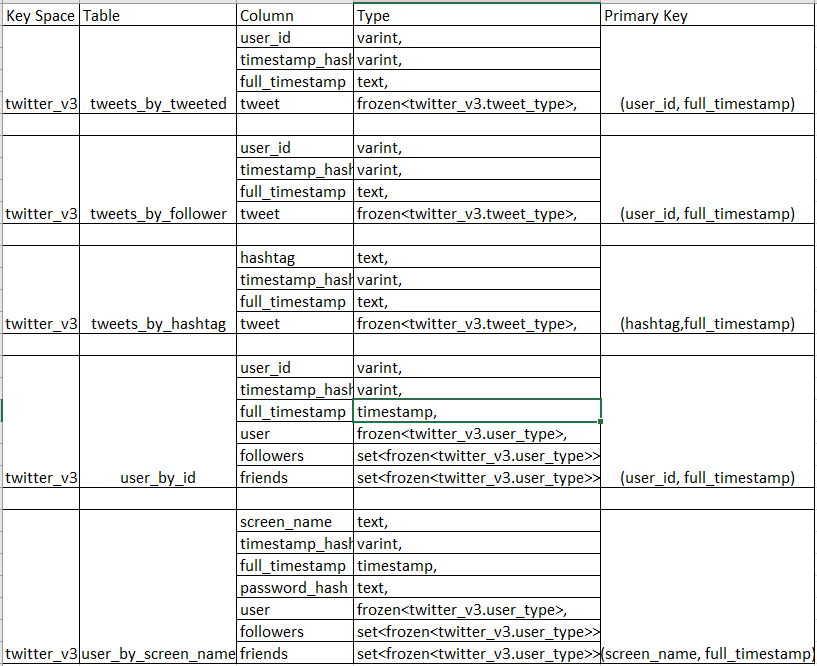
\includegraphics[scale=0.5, draft]{pics/schema.png}
	\caption{Cassandra Schema}
	\label{fig:schema}
\end{figure}
Da man bei Cassandra nur über den Primary Key (PK) auf Zeilen zugreifen und Bereichsabfragen über CQL machen kann, gilt es hier den PK so zu wählen, dass alle unsere Funktionen abgedeckt sind. Deshalb haben wir bei neben der User-Id für user\_by\_id und dem Screen-Name der Users für user\_by\_screen\_name auch den Timestamp mit aufgenommen. Da Cassandra leider keine vollständige Konsistenz bietet, müssen wir uns selber darum kümmern. Durch den Timestamp können wir verschiedene Versionen eines Objektes auseinander halten und die neuste bestimmen. Somit können wir zumindest einen gewissen Grad an Konsistenz bieten. Die weiteren Attribute der beiden Tabellen lassen sich einfach erklären. Die Follower und Friends eines Users sind wichtig, um die Timeline zu erstellen. Den password\_hash in user\_by\_screen\_name brauchen wir für den Login.\\
Die anderen drei Tabellen sind dafür da, die Tweets zu speichern und alle Tweet betreffenden Anfragen zu beantworten. Auch hier haben wir wieder den Timestamp bei allen Tabellen mit in den PK aufgenommen um Teilkonsistenz zu gewährleisten. tweets\_by\_tweeted speichert alle Tweets nach der User-Id des Users ab, der den Tweet abgesetzt hat. tweets\_by\_follower hingegen speichert einmal alle Tweets nach User-Id eines jeden Followers ab. Das Konzept hier ist es, durch die mehrfache Speicherung eines Tweets die Zeit bei der Abfrage nach allen Tweets, die ein User auf seiner Timeline sehen kann, zu verkürzen. Da man einmal abgesetzte Tweets auch nicht mehr ändern kann haben wir auch kein Problem damit jedes Objekt für Änderungen wieder heraussuchen zu müssen. tweets\_by\_hashtag speichert dann die Tweets danach ab, welche Hashtags in ihnen verwendet werden. Somit können auch Abfragen über Tweets eines Hashtags effizient beantwortet werden.

\section{Cassandrareader}
Die zentrale Applikation in der alle Funktionen und Schnittstellen umgesetzt werden ist der cassandrareader. Es ist eine modular aufgebaute in Java geschriebene Anwendung. Als Framework zur Unterstützung von verschiedenen Funktionen haben wir uns für SpringBoot entschieden. SpringBoot hat den Vorteil, dass es eine native API für Kafka besitzt, die es uns sehr leicht ermöglicht Publisher und Subscriber für Kafka-Topics zu schreiben. So ist die Verbindung mit Kafka sehr einfach konfigurierbar und kann innerhalb von kurzer Zeit verwendet werden. Für die Verbindung von Java zu Cassandra haben wir der DataStax Treiber genutzt \cite{DataStax}. Er biete eine generische Schnittstelle über die man mit Cassandra über CQL kommunizieren kann. Da er gut dokumentiert ist und es sehr viele Beispiele für verschiedene Anwendungen im Internet gibt, verlief die Einarbeitung in die Nutzung des DataStax Treibers sehr schnell.
\begin{figure}[htbp]
	\centering
	\includegraphics[scale=0.5, draft]{pics/cassandrareader_stack.png}
	\caption{Technologie Stack des cassandrareaders}
	\label{fig:techStackCass}
\end{figure}
Alle hier und im folgenden genutzten Bibliotheken werden über Maven eingebunden und der Applikation so zur Verfügung gestellt. Somit ist sichergestellt, dass immer die richtige Version geladen wird und keine Kompatibilitätsprobleme entstehen.

\subsection{Architektur}
Der Aufbau des Cassandrareaders ist sehr einfach gehalten wie man in Abbildung \ref{fig:archCass} sehen. Die Verbindung zu Cassandra wird vom Singleton CassandraConnector gemanaged. Diese Klasse stellt die Verbindung zu Cassandra her und bietet verschiedene Methoden an, Abfragen an Cassandra über CQL abzusetzen. Die eigentlich Funktion und Implementierung der Use Cases geschieht aber in den Kafka Subscribern. Dazu gibt es eine abstrakte Klasse AbstractKafkaSubscriber, die sozusagen die Infrastruktur bereitstellt. Diese besteht aus dem CassandraConnector, eine Gson-Instanz und mehreren Methoden, die die Optimierungen der Methoden aus dem Cassandra Connector darstellen, wie z.B. Batch-Queries und asynchrone Queries. Die Gson-Instanz kommt von der Google Gson Bibliothek, die für die JSON Konvertierung von Java Klasse zuständig ist. Sie wird in den abgeleiteten Klassen so benutzt, dass Kafka-Anfragen direkt in POJO Objekte gemappt werden, aus denen man dann alle relevanten Informationen bekommt. In den abgeleiteten Klassen wird dann auch die eigentliche Funktion eines Use Cases implementiert.
\begin{figure}[htbp]
	\centering
	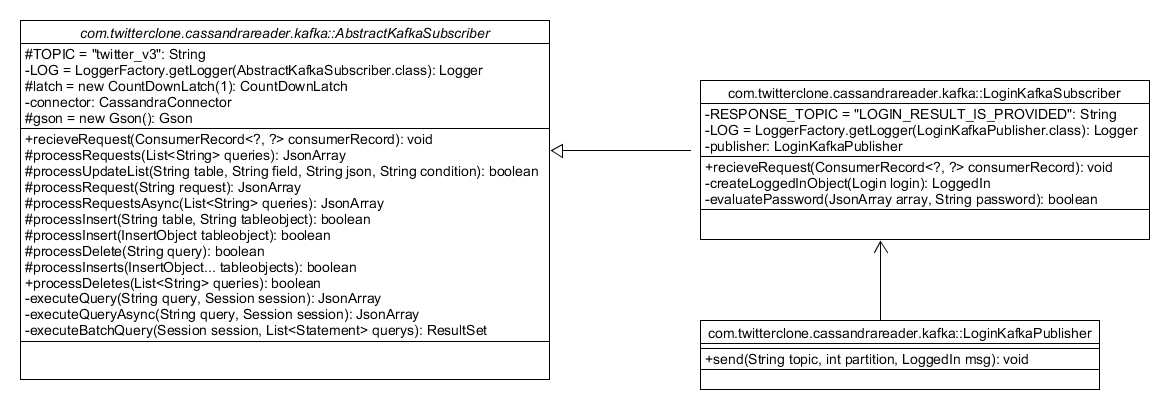
\includegraphics[scale=0.25, draft]{pics/cassandrareader_architecture.png}
	\caption{Technologie Stack des cassandrareaders}
	\label{fig:archCass}
\end{figure}
Alle möglichen Anfragen und Antworten über Kafka sind als Java Klassen modelliert und können über Getter-Methoden abgefragt werden. Jeder der abgeleiteten Subscriber besitzt einen Publisher, über den die Antwort, durch Gson konvertiert, wieder versendet werden kann. Die Konfigurationsparameter sind in der application.properties abgelegt und werden in den einzelnen Klassen angesprochen.


\section{Use Cases}
\label{sec:usecase}
Bei der Identifizierung der Use Cases die für Cassandra relevant sind haben wir uns für die Funktionen entschieden, die für einen Twitter-Client nach MVP-Prinzip (Minimal Viable Product) notwendig sind. Dabei haben wir vor allem die dazu gehören folgende Funktionen:
\begin{itemize}
	\item Registrierung von User
	\item Anmelden von Usern
	\item Abrufen der Timeline:
		\begin{itemize}
			\item Abfragen von Tweets
			\item Abfragen von Usern
		\end{itemize}
	\item Absenden/Speichern von Tweets
\end{itemize}
Diese Schnittstellen machen es möglich die Grundfunktionen, also das Erstellen eines Users, das Anmelden, das Senden von Tweets und das Lesen von Tweets über die Timeline von außen über vordefinierte Kafka Nachrichten anzusprechen.
Als weitere Schnittstellen für erweiterte Funktionen haben wir eine API für Volltextsuche über Elasticsearch gebaut, die die normale Volltextsuche aber auch Autocompletion unterstützt.\\ \TODO{vielleicht deletion hinzufügen}




\subsection{Registrierung von Usern}

\subsection{Anmelden von Usern}

\subsection{Abfragen von Tweets}

\subsection{Abfragen von Usern}

\subsection{Abrufen der Timeline}

\subsection{Absenden/Speichern von Tweets}



\chapter{Implementation}

\section{Architecture}










\chapter{Evaluation}

\section{Experiments}

\section{Results}
\chapter{Conclusion}
Write here you conclusions

\section{Future work}




\blankpage

% usare questo invece di usare \appendix perchè l'altro dà un ref sbagliato sul primo link dell'indice
\begin{appendices}
	\chapter{Glossary}
\label{appendixA}
Just comment \verb|\chapter{Glossary}
\label{appendixA}
Just comment \verb|\chapter{Glossary}
\label{appendixA}
Just comment \verb|\input{AppendixA-Glossary.tex}| in Masterthesis.tex if you don't need it!

\begin{longtable}{p{2.5cm}p{9.5cm}}

\huge{\textbf{Symbols}}& \\
\hline
\\
\$ & US. dollars. \\
\\
\\
\huge{\textbf{A}}& \\
\hline
\\
A& Meaning of A.\\
\\
\\
\huge{\textbf{B}}& \\
\hline
\\

\\
\\
\huge{\textbf{C}}& \\
\hline
\\

\\
\\
\huge{\textbf{D}}& \\
\hline
\\

\\
\\
\huge{\textbf{E}}& \\
\hline
\\

\\
\\
\huge{\textbf{F}}& \\
\hline
\\

\\
\\
\huge{\textbf{G}}& \\
\hline
\\
\\
\\
\huge{\textbf{H}}& \\
\hline
\\

\\
\\
\huge{\textbf{I}}& \\
\hline
\\

\\
\\
\huge{\textbf{J}}& \\
\hline
\\

\\
\\
%\huge{\textbf{K}}& \\
%\hline
%\\
%\\
%\\
%\huge{\textbf{L}}& \\
%\hline
%\\
%\\
%\\
\huge{\textbf{M}}& \\
\hline
\\

\\
\\
\huge{\textbf{N}}& \\
\hline
\\

\\
\\
%\huge{\textbf{O}}& \\
%\hline
%\\
%\\
%\\
\huge{\textbf{P}}& \\
\hline
\\

\\
\\
\huge{\textbf{Q}}& \\
\hline
\\

\\
\\
\huge{\textbf{R}}& \\
\hline
\\

\\
\\
\huge{\textbf{S}}& \\
\hline
\\

\\
\\
\huge{\textbf{T}}& \\
\hline
\\

\\
\\
\huge{\textbf{U}}& \\
\hline
\\

\\
\\
\huge{\textbf{V}}& \\
\hline
\\

\\
\\
\huge{\textbf{W}}& \\
\hline
\\

\\
\\
\huge{\textbf{X}}& \\
\hline
\\

\\
\\
%\huge{\textbf{Y}}& \\
%\hline
%\\
%\\
%\\
%\huge{\textbf{Z}}& \\
%\hline
%\\
%\\
%\\
\end{longtable}



| in Masterthesis.tex if you don't need it!

\begin{longtable}{p{2.5cm}p{9.5cm}}

\huge{\textbf{Symbols}}& \\
\hline
\\
\$ & US. dollars. \\
\\
\\
\huge{\textbf{A}}& \\
\hline
\\
A& Meaning of A.\\
\\
\\
\huge{\textbf{B}}& \\
\hline
\\

\\
\\
\huge{\textbf{C}}& \\
\hline
\\

\\
\\
\huge{\textbf{D}}& \\
\hline
\\

\\
\\
\huge{\textbf{E}}& \\
\hline
\\

\\
\\
\huge{\textbf{F}}& \\
\hline
\\

\\
\\
\huge{\textbf{G}}& \\
\hline
\\
\\
\\
\huge{\textbf{H}}& \\
\hline
\\

\\
\\
\huge{\textbf{I}}& \\
\hline
\\

\\
\\
\huge{\textbf{J}}& \\
\hline
\\

\\
\\
%\huge{\textbf{K}}& \\
%\hline
%\\
%\\
%\\
%\huge{\textbf{L}}& \\
%\hline
%\\
%\\
%\\
\huge{\textbf{M}}& \\
\hline
\\

\\
\\
\huge{\textbf{N}}& \\
\hline
\\

\\
\\
%\huge{\textbf{O}}& \\
%\hline
%\\
%\\
%\\
\huge{\textbf{P}}& \\
\hline
\\

\\
\\
\huge{\textbf{Q}}& \\
\hline
\\

\\
\\
\huge{\textbf{R}}& \\
\hline
\\

\\
\\
\huge{\textbf{S}}& \\
\hline
\\

\\
\\
\huge{\textbf{T}}& \\
\hline
\\

\\
\\
\huge{\textbf{U}}& \\
\hline
\\

\\
\\
\huge{\textbf{V}}& \\
\hline
\\

\\
\\
\huge{\textbf{W}}& \\
\hline
\\

\\
\\
\huge{\textbf{X}}& \\
\hline
\\

\\
\\
%\huge{\textbf{Y}}& \\
%\hline
%\\
%\\
%\\
%\huge{\textbf{Z}}& \\
%\hline
%\\
%\\
%\\
\end{longtable}



| in Masterthesis.tex if you don't need it!

\begin{longtable}{p{2.5cm}p{9.5cm}}

\huge{\textbf{Symbols}}& \\
\hline
\\
\$ & US. dollars. \\
\\
\\
\huge{\textbf{A}}& \\
\hline
\\
A& Meaning of A.\\
\\
\\
\huge{\textbf{B}}& \\
\hline
\\

\\
\\
\huge{\textbf{C}}& \\
\hline
\\

\\
\\
\huge{\textbf{D}}& \\
\hline
\\

\\
\\
\huge{\textbf{E}}& \\
\hline
\\

\\
\\
\huge{\textbf{F}}& \\
\hline
\\

\\
\\
\huge{\textbf{G}}& \\
\hline
\\
\\
\\
\huge{\textbf{H}}& \\
\hline
\\

\\
\\
\huge{\textbf{I}}& \\
\hline
\\

\\
\\
\huge{\textbf{J}}& \\
\hline
\\

\\
\\
%\huge{\textbf{K}}& \\
%\hline
%\\
%\\
%\\
%\huge{\textbf{L}}& \\
%\hline
%\\
%\\
%\\
\huge{\textbf{M}}& \\
\hline
\\

\\
\\
\huge{\textbf{N}}& \\
\hline
\\

\\
\\
%\huge{\textbf{O}}& \\
%\hline
%\\
%\\
%\\
\huge{\textbf{P}}& \\
\hline
\\

\\
\\
\huge{\textbf{Q}}& \\
\hline
\\

\\
\\
\huge{\textbf{R}}& \\
\hline
\\

\\
\\
\huge{\textbf{S}}& \\
\hline
\\

\\
\\
\huge{\textbf{T}}& \\
\hline
\\

\\
\\
\huge{\textbf{U}}& \\
\hline
\\

\\
\\
\huge{\textbf{V}}& \\
\hline
\\

\\
\\
\huge{\textbf{W}}& \\
\hline
\\

\\
\\
\huge{\textbf{X}}& \\
\hline
\\

\\
\\
%\huge{\textbf{Y}}& \\
%\hline
%\\
%\\
%\\
%\huge{\textbf{Z}}& \\
%\hline
%\\
%\\
%\\
\end{longtable}



\blankpage
	\chapter{Appendix}
\label{appendixB}
\section{Something you need in the appendix}
Just comment \verb|\chapter{Appendix}
\label{appendixB}
\section{Something you need in the appendix}
Just comment \verb|\chapter{Appendix}
\label{appendixB}
\section{Something you need in the appendix}
Just comment \verb|\input{AppendixB.tex}| in Masterthesis.tex if you don't need it!| in Masterthesis.tex if you don't need it!| in Masterthesis.tex if you don't need it!
	%\chapter{Appendix C}
\label{appendiceC}
Some text.

\section{Section 1}

\section{Section 2}
	%\chapter{Appendix D}

\section{Section 1}

\end{appendices}

%Declaration
\pagestyle{empty}
\newpage
\section*{Erklärung}

Hiermit erkläre ich, dass ich diese Abschlussarbeit selbständig verfasst
habe, keine anderen als die angegebenen Quellen/Hilfsmittel verwendet
habe und alle Stellen, die wörtlich oder sinngemäß aus veröffentlichten
Schriften entnommen wurden, als solche kenntlich gemacht habe. Darüber
hinaus erkläre ich, dass diese Abschlussarbeit nicht, auch nicht auszugsweise,
bereits für eine andere Prüfung angefertigt wurde.\\
\begin{tabular}{lp{3em}l}
\vspace{1cm}
 \hspace{6cm}   && \hspace{6cm} \\\cline{1-1}\cline{3-3}
 Ort, Datum     && Unterschrift
\end{tabular}

% Esempio
%\index{Esempio |see{Esempio 2}}

\blankpage

%Indice analitico per il momento non verra' messo.
%\printindex %indice analitico

\bibliography{references}
\end{document}

%comandi utilizzati nel template:
%\texttt{} %per scrivere con carattere diverso
%\textbf{} %per scrivere con carattere diverso
%\href{http://www.blob.com/}{testo}
%\index{} %per indice analitico
%\footnote{} %note
%\noindent 
%\label{} 
%\ref{}
%\cite{PdfReference}
%\bibitem{PdfReference}
%®
%
%per inserire una figura:
%\begin{figure}[H]
%\begin{center}
%\includegraphics[width=12cm]{problematiche-del-ciclo-passivo.eps}\\
%\caption{Ciclo attivo e passivo in un'azienda}
%\label{fig:cicliAziendali}
%\end{center}
%\end{figure}
%
%per inserire una tabella:
%\begin{longtable}{p{3cm}p{9cm}}
%\textbf{Titolo} & Descrizione.\\
%\\
%\textbf{Titolo} & Descrizione.\\
%\\
%\end{longtable}
